\documentclass[../rapport.tex]{subfiles}
\graphicspath{{\subfix{ressources/photos_diagrammes/app1/}}}

\usepackage[utf8]{inputenc}
\usepackage[french]{babel}
\usepackage{amsmath, amsfonts, amssymb, amsthm}

\begin{document}
\begin{enumerate}
	\item{Accéder à la liste des portefeuilles}\\
			\begin{figure}[h]
				\centering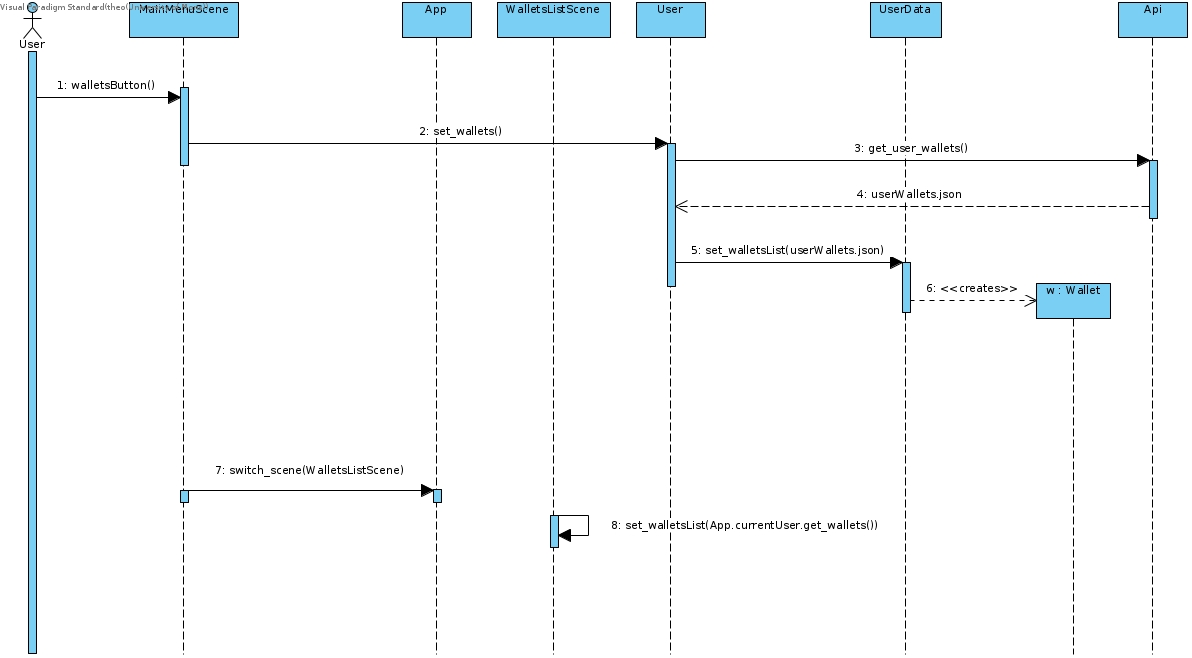
\includegraphics[scale=0.25]{ressources/photos_diagrammes/app1/sequences/accederPortefeuilles.jpg}
				\caption{Accéder à la liste des portefeuilles}
			\end{figure}	
Ce diagrammes de séquences décrit comment l'application va récupérer la liste des portefeuilles de l'utilisateur et la stocker au seins de l'application.
L'application va ensuite changer de scène pour passer sur l'écran d'affichage des portefeuilles. Cette scène pourra alors accéder facilement à la liste des portefeuilles afin de les afficher à l'utilisateur.
\newpage	
\item{Accéder à la liste des produits financiers}\\
			\begin{figure}[h]
				\centering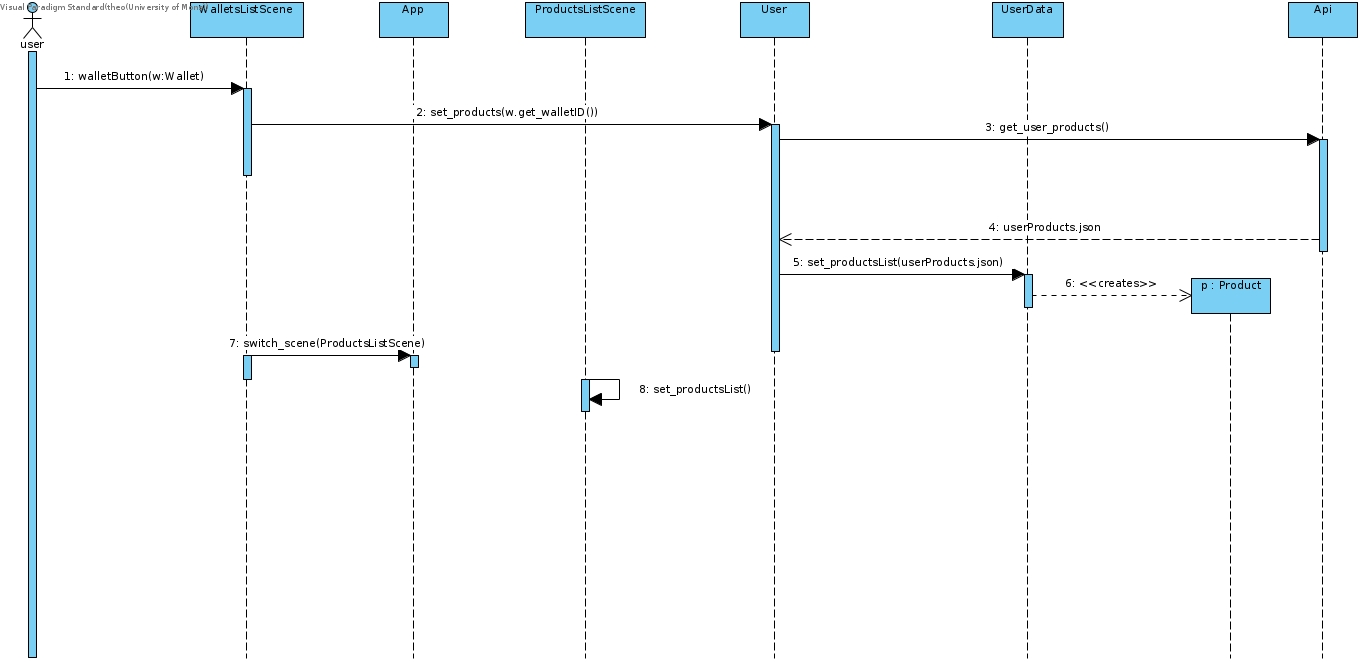
\includegraphics[scale=0.25]{ressources/photos_diagrammes/app1/sequences/accederProduits.jpg}
				\caption{Accéder à la liste des produits financiers}
			\end{figure}	
Lorsque l'utilisateur sélectionne un de ses portefeuilles, les produits financiers de ce portefeuilles doivent être récupérés depuis le serveur. Ils sont ensuite stockés dans une liste de l'objet Wallet. Une fois les produits récupérés, la scène des détails d'un portefeuille est affichée.
\newpage	
		\item{Créer un compte}\\
			\begin{figure}[h]
				\centering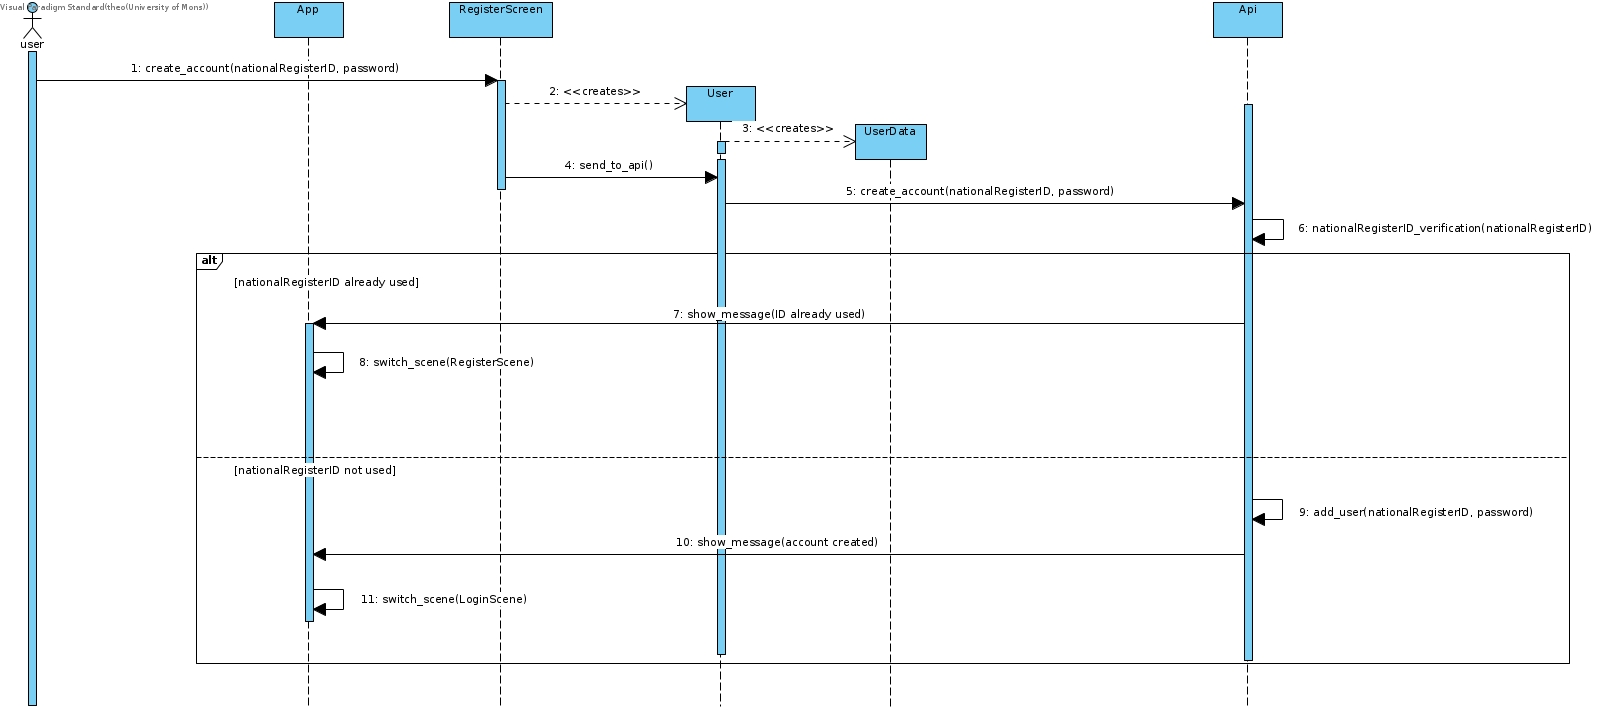
\includegraphics[scale=0.25]{ressources/photos_diagrammes/app1/sequences/creerCompte.jpg}
				\caption{Créer un compte}
			\end{figure}	
Afin de créer un compte, l'utilisateur va entrer ses données qui seront ensuite utilisées afin de créer un objet UserData. Cet objet va ensuite être envoyé vers le serveur sous forme d'un fichier json.
\newpage	
		\item{Créer un portefeuille}\\
			\begin{figure}[h]
				\centering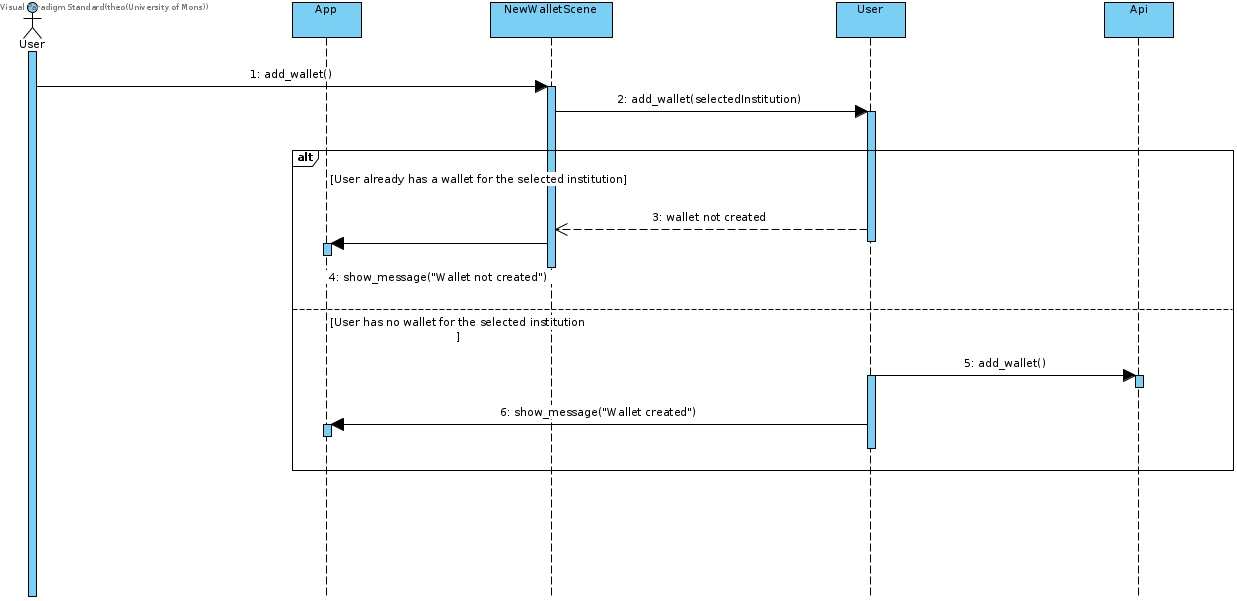
\includegraphics[scale=0.25]{ressources/photos_diagrammes/app1/sequences/creerPortefeuille.jpg}
				\caption{Créer un portefeuille}
			\end{figure}	
La création d'un portefeuille demande peu d'informations à l'utilisateur. Une fois qu'il a selectionné l'institution pour laquelle il veut créer un portefeuille, l'application va vérifier si il a déjà un portefeuille pour cette institution. Si c'est le cas, une notification d'erreur lui sera affichée. Sinon le portefeuille sera créé et l'information sera envoyée vers le serveur.
\newpage	
		\item{Effectuer une transaction}\\
			\begin{figure}[h]
				\centering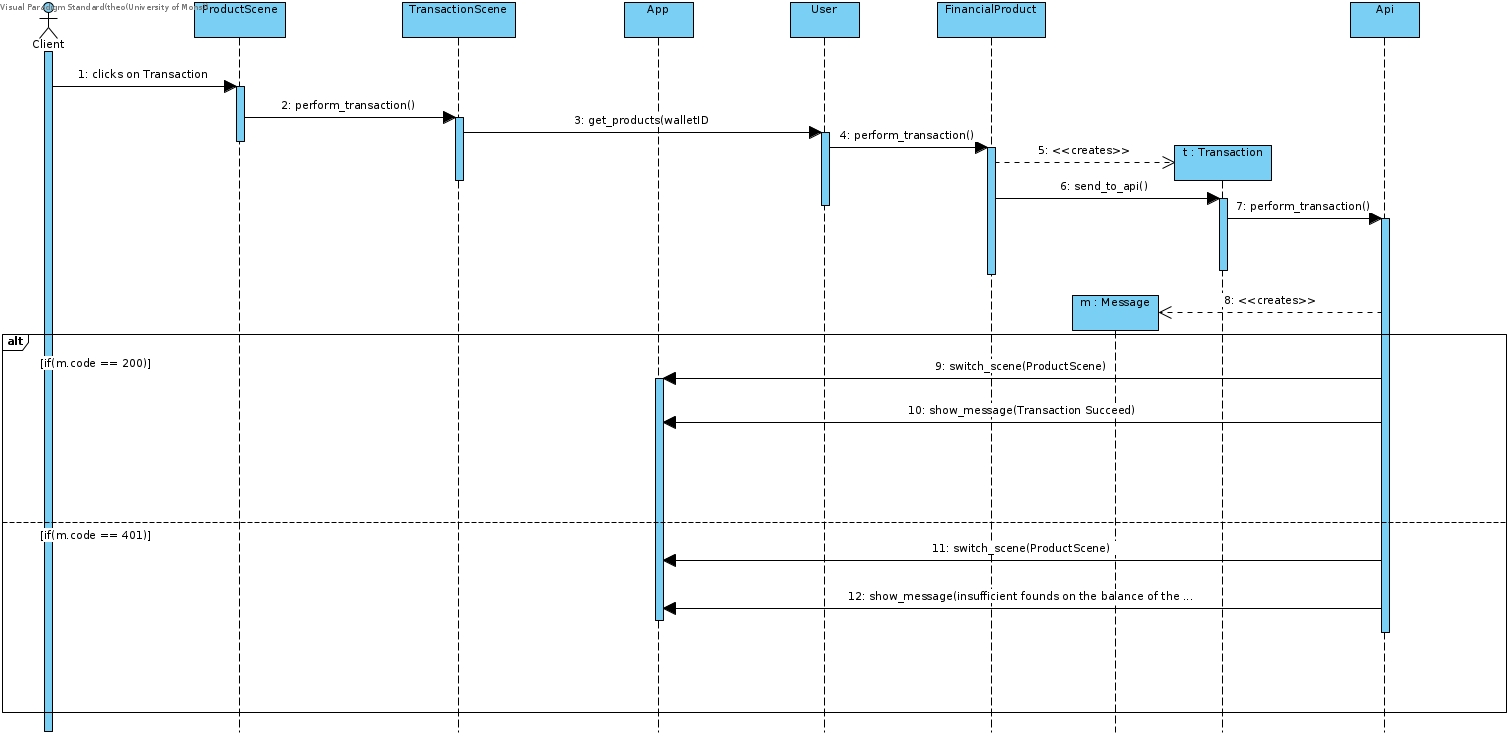
\includegraphics[scale=0.25]{ressources/photos_diagrammes/app1/sequences/effectuerTrx.jpg}
				\caption{Effectuer une transaction}
			\end{figure}	
Une fois que l'utilisateur a entré les informations de la transaction et accepté la confirmation, un objet Transaction est créé et envoyé vers le serveur.
\newpage	
		\item{Se connecter}\\
			\begin{figure}[h]
				\centering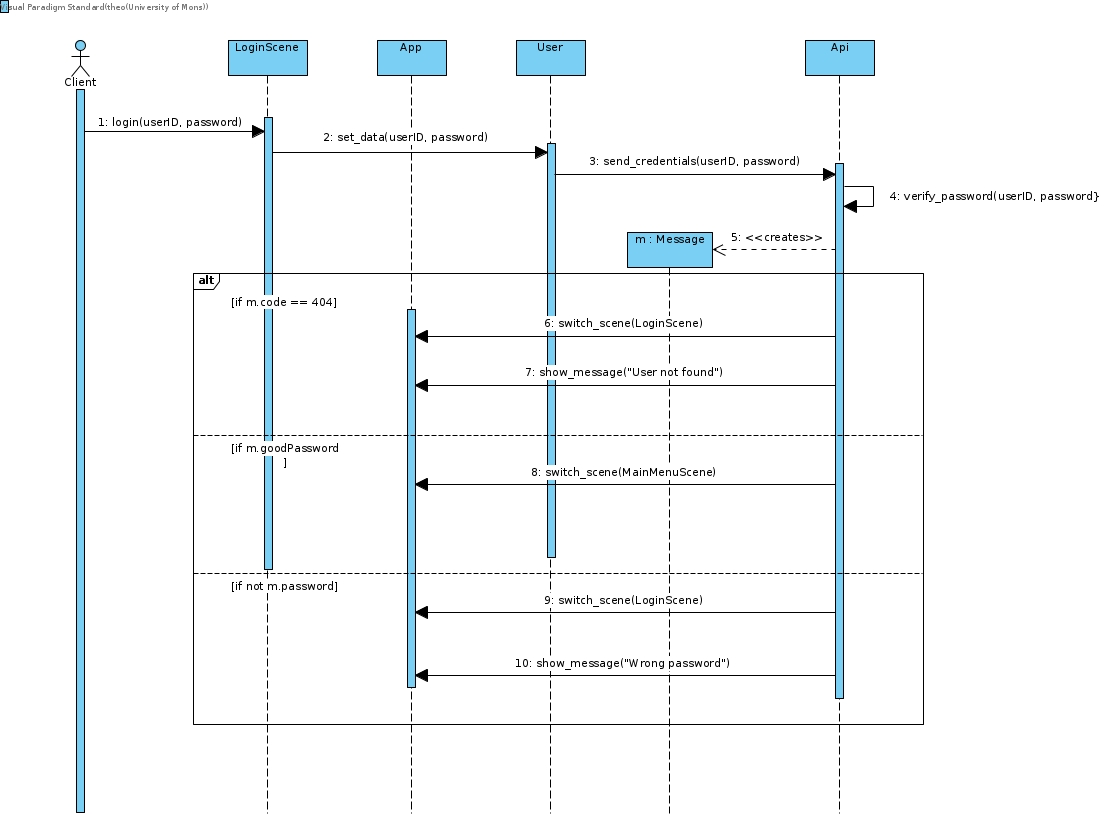
\includegraphics[scale=0.3]{ressources/photos_diagrammes/app1/sequences/connecter.jpg}
				\caption{Se connecter}
			\end{figure}	
La procédure de connexion à l'app est initiée lorque l'utilisateur entre ses identifiants et clique sur se connecter. Ses identifiants seront alors envoyés à l'api qui verfiera ceux-ci. Si ils sont corrects alors l'utilisateur est envoyé vers le menu principal de l'application. Si le nom d'utilisateur et incorrect un message ``user not found'' lui est affiché et si le mot de passe est incorrect alors un message ``wrong password'' est affiché.
\newpage	
		\item{Souscrire à un produit financier}\\
			\begin{figure}[h]
				\centering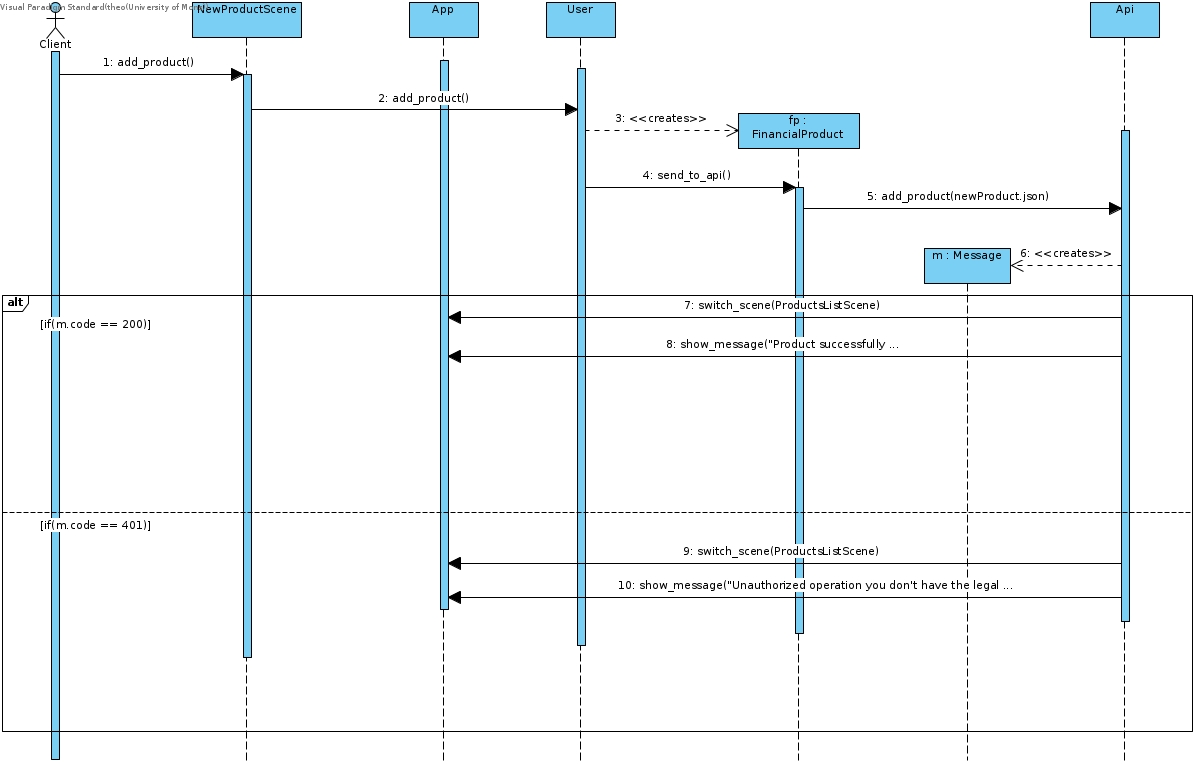
\includegraphics[scale=0.3]{ressources/photos_diagrammes/app1/sequences/souscrireProduit.jpg}
				\caption{Souscrire à un produit financier}
			\end{figure}	
Lorqu'un produit financié est créé par l'utilisateur, cela envoie un objet FinancialProduct à l'api qui se chargera de l'envoyer vers le serveur.
Un message est ensuite envoyé à l'utilisateur afin de l'informer de la réussite (ou échec) de l'opération.
\newpage
\end{enumerate}
\end{document}

